
\documentclass[border=10pt, 12pt]{standalone}
\usepackage[svgnames]{xcolor}
\usepackage{amsmath}
\usepackage{pgfplots}
\pgfplotsset{compat=newest}
\usepackage[sfdefault]{FiraSans}
\usepackage{FiraMono}
\renewcommand*\familydefault{\sfdefault}
\begin{document}
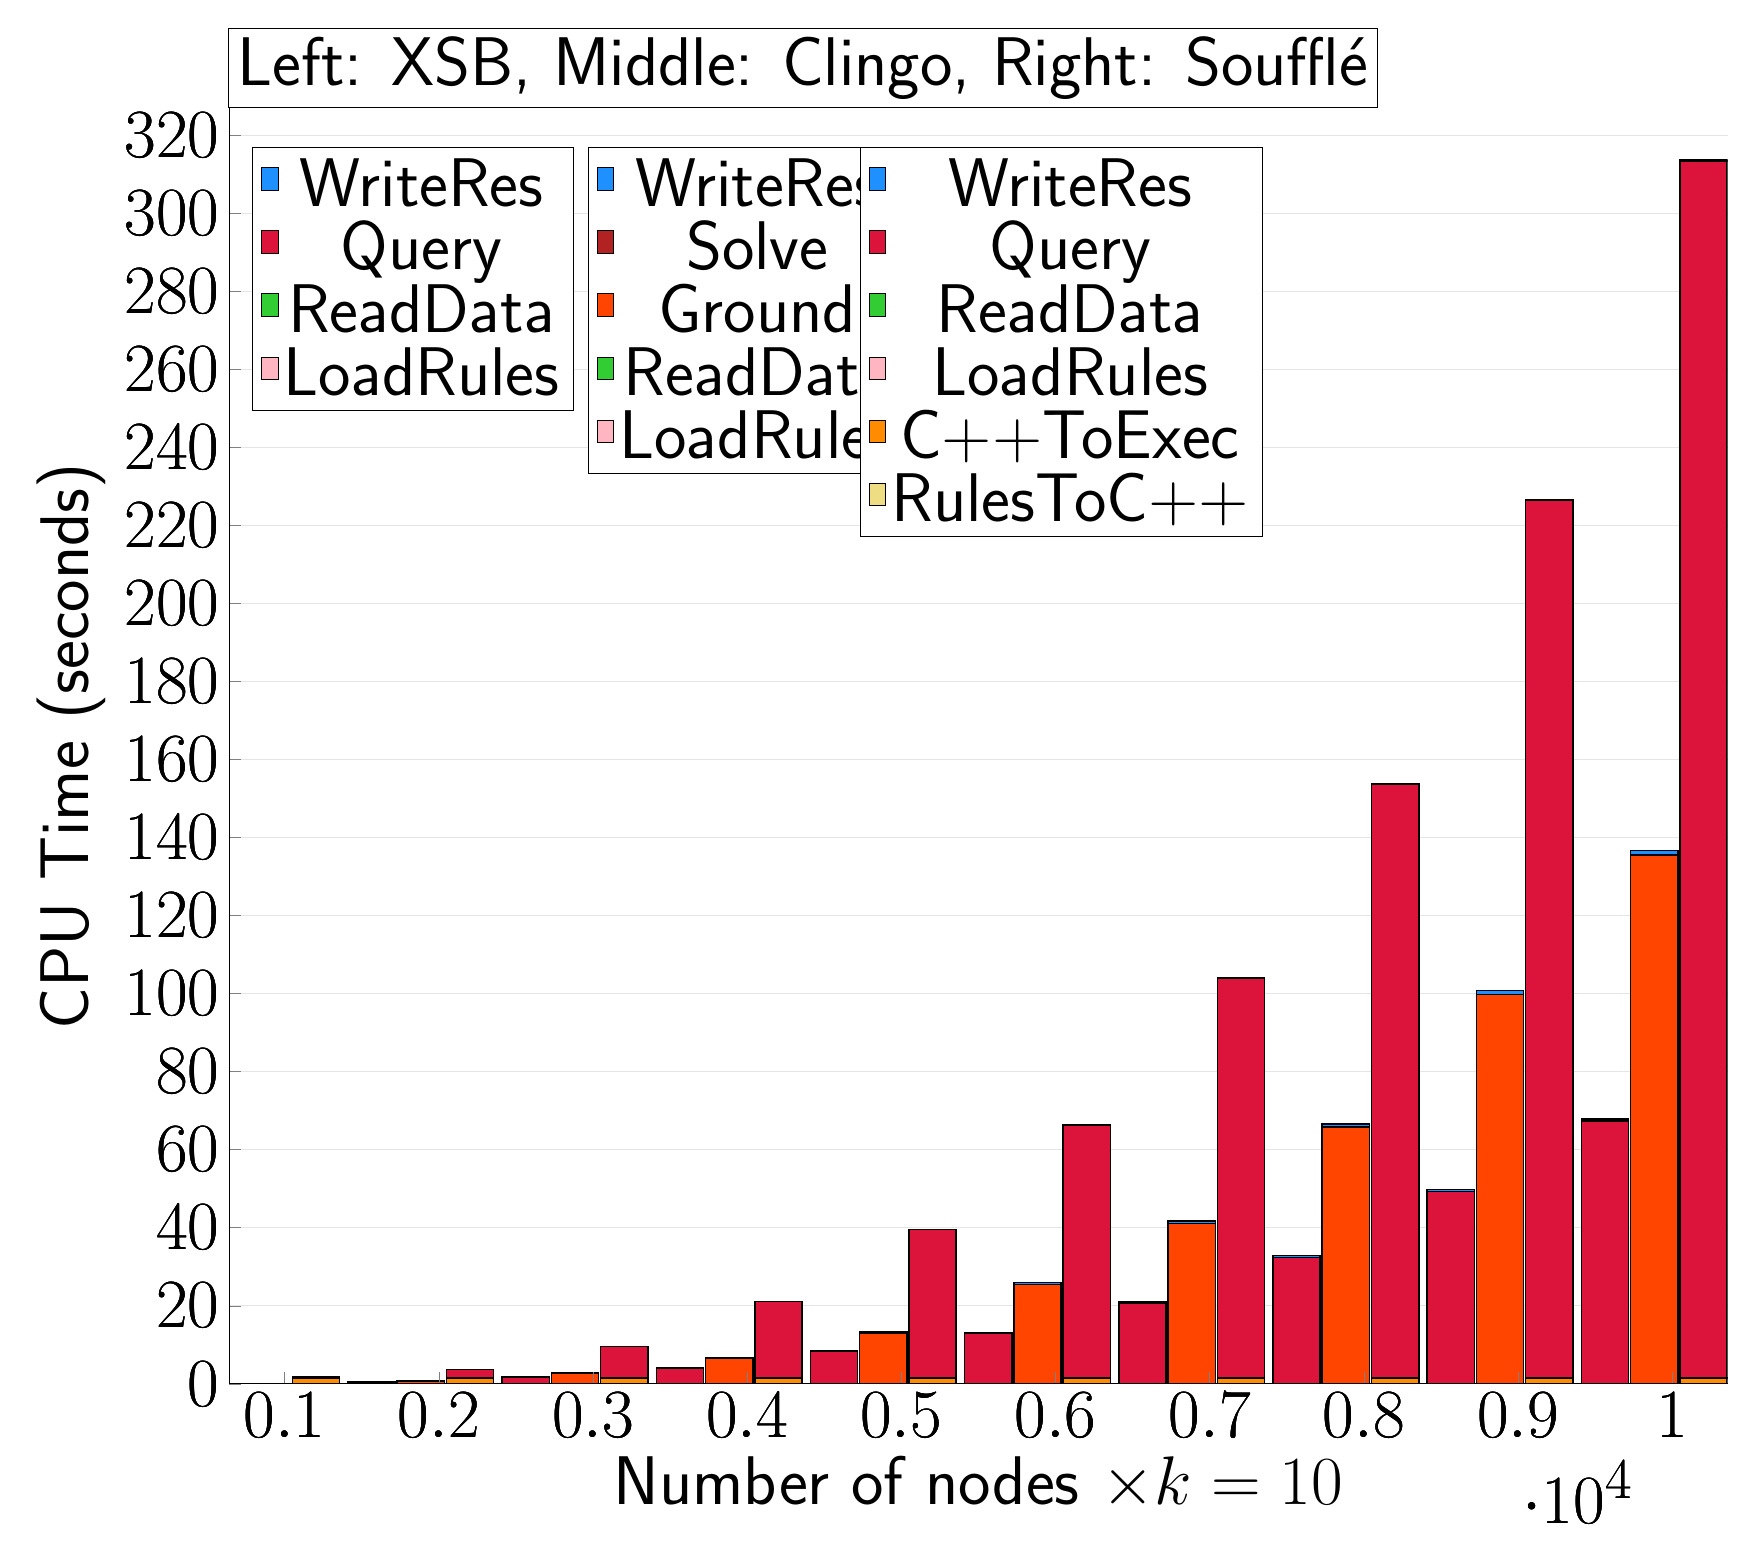
\begin{tikzpicture}
                        \begin{axis}[bar shift=-24.3pt, 
   ybar stacked,
   width=1.7\textwidth,
   bar width=0.6cm,
   ymajorgrids, tick align=inside,
   major grid style={draw=gray!20},
   xtick=data,
   ymin=0, ymax=326.9108,
   axis x line*=bottom,
   axis y line*=left,
   enlarge x limits=0.04,
   legend style={
       at={(0.23, 0.97)},
       anchor=north east,
       legend columns=1,
       font=\Huge,
   },
   ylabel={CPU Time (seconds)},
   xlabel={Number of nodes $\times k=10$},
   label style={font=\Huge},
   tick label style={font=\Huge},
]
\addlegendimage{fill=DodgerBlue, draw=black, line width=0.2pt}
\addlegendentry{WriteRes}
\addlegendimage{fill=Crimson, draw=black, line width=0.2pt}
\addlegendentry{Query}
\addlegendimage{fill=LimeGreen, draw=black, line width=0.2pt}
\addlegendentry{ReadData}
\addlegendimage{fill=LightPink, draw=black, line width=0.2pt}
\addlegendentry{LoadRules}
\addplot +[fill=LightPink, draw=black, line width=0.55pt] coordinates {
(1000, 0.0005609999999999998)
(2000, 0.0005557999999999995)
(3000, 0.0005511999999999997)
(4000, 0.0005546000000000006)
(5000, 0.0005583999999999994)
(6000, 0.0005632)
(7000, 0.0005550000000000002)
(8000, 0.0005597999999999998)
(9000, 0.0005571999999999998)
(10000, 0.0005519999999999995)
};
\addplot +[fill=LimeGreen, draw=black, line width=0.55pt] coordinates {
(1000, 0.0009510000000000008)
(2000, 0.0018281999999999999)
(3000, 0.002706)
(4000, 0.0035464000000000003)
(5000, 0.0044942)
(6000, 0.0053516)
(7000, 0.006229800000000001)
(8000, 0.007026200000000001)
(9000, 0.007960199999999999)
(10000, 0.0088426)
};
\addplot +[fill=Crimson, draw=black, line width=0.55pt] coordinates {
(1000, 0.0577216)
(2000, 0.49301340000000005)
(3000, 1.6136984)
(4000, 3.9585594)
(5000, 8.4288846)
(6000, 12.865281200000002)
(7000, 20.7034066)
(8000, 32.368014800000005)
(9000, 49.3121658)
(10000, 67.3184562)
};
\addplot +[fill=DodgerBlue, draw=black, line width=0.55pt] coordinates {
(1000, 0.00794)
(2000, 0.03468340000000001)
(3000, 0.06950920000000002)
(4000, 0.11473979999999981)
(5000, 0.1550903999999999)
(6000, 0.2390199999999993)
(7000, 0.4243060000000007)
(8000, 0.4717049999999965)
(9000, 0.4649876000000006)
(10000, 0.5109529999999978)
};
\end{axis}

\begin{axis}[bar shift=-6.5pt, 
   ybar stacked,
   width=1.7\textwidth,
   bar width=0.6cm,
   ymajorgrids, tick align=inside,
   major grid style={draw=none},
   xtick=data,
   ymin=0, ymax=326.9108,
   axis x line*=none,
   axis y line*=none,
   enlarge x limits=0.04,
   legend style={
       at={(0.454, 0.97)},
       anchor=north east,
       legend columns=1,
       font=\Huge,
   },
   label style={font=\Huge},
   tick label style={font=\Huge},
]
\addlegendimage{fill=DodgerBlue, draw=black, line width=0.2pt}
\addlegendentry{WriteRes}
\addlegendimage{fill=FireBrick, draw=black, line width=0.2pt}
\addlegendentry{Solve}
\addlegendimage{fill=OrangeRed, draw=black, line width=0.2pt}
\addlegendentry{Ground}
\addlegendimage{fill=LimeGreen, draw=black, line width=0.2pt}
\addlegendentry{ReadData}
\addlegendimage{fill=LightPink, draw=black, line width=0.2pt}
\addlegendentry{LoadRules}
\addplot +[fill=LightPink, draw=black, line width=0.55pt] coordinates {
(1000, 0.0)
(2000, 0.0)
(3000, 0.0)
(4000, 0.0)
(5000, 0.0)
(6000, 0.0)
(7000, 0.0)
(8000, 0.0)
(9000, 0.0)
(10000, 0.0)
};
\addplot +[fill=LimeGreen, draw=black, line width=0.55pt] coordinates {
(1000, 0.0)
(2000, 0.0)
(3000, 0.0)
(4000, 0.010000000000000009)
(5000, 0.010000000000000009)
(6000, 0.010000000000000009)
(7000, 0.01200000000000001)
(8000, 0.018000000000000016)
(9000, 0.020000000000000018)
(10000, 0.020000000000000018)
};
\addplot +[fill=OrangeRed, draw=black, line width=0.55pt] coordinates {
(1000, 0.10000000000000005)
(2000, 0.78)
(3000, 2.694)
(4000, 6.465999999999999)
(5000, 12.978)
(6000, 25.484)
(7000, 41.068000000000005)
(8000, 65.75999999999999)
(9000, 99.78399999999999)
(10000, 135.46200000000002)
};
\addplot +[fill=FireBrick, draw=black, line width=0.55pt] coordinates {
(1000, 0.0019999999999999905)
(2000, 0.0)
(3000, 0.009999999999999962)
(4000, 0.008000000000000184)
(5000, 0.011999999999999744)
(6000, 0.020000000000000285)
(7000, 0.029999999999999714)
(8000, 0.03800000000000421)
(9000, 0.0460000000000008)
(10000, 0.061999999999998404)
};
\addplot +[fill=DodgerBlue, draw=black, line width=0.55pt] coordinates {
(1000, 0.007999999999999974)
(2000, 0.050000000000000044)
(3000, 0.10599999999999991)
(4000, 0.18799999999999972)
(5000, 0.3000000000000005)
(6000, 0.4279999999999995)
(7000, 0.5759999999999996)
(8000, 0.7379999999999937)
(9000, 0.9400000000000002)
(10000, 1.1480000000000055)
};
\end{axis}

\begin{axis}[bar shift=11.3pt, 
   ybar stacked,
   width=1.7\textwidth,
   bar width=0.6cm,
   ymajorgrids, tick align=inside,
   major grid style={draw=none},
   xtick=data,
   ymin=0, ymax=326.9108,
   axis x line*=none,
   axis y line*=none,
   enlarge x limits=0.04,
   legend style={
       at={(0.69, 0.97)},
       anchor=north east,
       legend columns=1,
       font=\Huge,
   },
   label style={font=\Huge},
   tick label style={font=\Huge},
]
\addlegendimage{fill=DodgerBlue, draw=black, line width=0.2pt}
\addlegendentry{WriteRes}
\addlegendimage{fill=Crimson, draw=black, line width=0.2pt}
\addlegendentry{Query}
\addlegendimage{fill=LimeGreen, draw=black, line width=0.2pt}
\addlegendentry{ReadData}
\addlegendimage{fill=LightPink, draw=black, line width=0.2pt}
\addlegendentry{LoadRules}
\addlegendimage{fill=DarkOrange, draw=black, line width=0.2pt}
\addlegendentry{C++ToExec}
\addlegendimage{fill=LightGoldenrod, draw=black, line width=0.2pt}
\addlegendentry{RulesToC++}
\addplot +[fill=LightGoldenrod, draw=black, line width=0.55pt] coordinates {
(1000, 0.008000000000000002)
(2000, 0.004000000000000001)
(3000, 0.008000000000000002)
(4000, 0.011999999999999999)
(5000, 0.004000000000000001)
(6000, 0.006000000000000001)
(7000, 0.0020000000000000005)
(8000, 0.0)
(9000, 0.0020000000000000005)
(10000, 0.003999999999999997)
};
\addplot +[fill=DarkOrange, draw=black, line width=0.55pt] coordinates {
(1000, 1.482)
(2000, 1.486)
(3000, 1.4540000000000002)
(4000, 1.456)
(5000, 1.464)
(6000, 1.456)
(7000, 1.468)
(8000, 1.474)
(9000, 1.474)
(10000, 1.484)
};
\addplot +[fill=LightPink, draw=black, line width=0.55pt] coordinates {
(1000, 0.0001734)
(2000, 0.00018779999999999998)
(3000, 0.00019160000000000002)
(4000, 7.999999999999999e-05)
(5000, 0.0001558)
(6000, 0.00010040000000000001)
(7000, 0.0001712)
(8000, 0.0001494)
(9000, 0.0002134)
(10000, 0.00018839999999999997)
};
\addplot +[fill=LimeGreen, draw=black, line width=0.55pt] coordinates {
(1000, 0.0042642)
(2000, 0.005886)
(3000, 0.0087968)
(4000, 0.0080006)
(5000, 0.0143382)
(6000, 0.011474599999999998)
(7000, 0.018571200000000003)
(8000, 0.0201148)
(9000, 0.025695000000000003)
(10000, 0.029549799999999998)
};
\addplot +[fill=Crimson, draw=black, line width=0.55pt] coordinates {
(1000, 0.31416180000000005)
(2000, 2.208696)
(3000, 8.112143999999999)
(4000, 19.619419999999998)
(5000, 38.01953999999999)
(6000, 64.90376)
(7000, 102.46020000000001)
(8000, 152.1612)
(9000, 224.9568)
(10000, 311.9108)
};
\addplot +[fill=DodgerBlue, draw=black, line width=0.55pt] coordinates {
(1000, 0.002498)
(2000, 0.008849200000000002)
(3000, 0.019813000000000004)
(4000, 0.0349328)
(5000, 0.0540492)
(6000, 0.0775386)
(7000, 0.10575280000000001)
(8000, 0.13568960000000002)
(9000, 0.1721598)
(10000, 0.2114398)
};
\end{axis}


\node[anchor=south, draw, fill=white] at (rel axis cs:0.42,1) {\Huge Left: XSB, Middle: Clingo, Right: Soufflé};
\end{tikzpicture}
\end{document}
                    